\documentclass[a4paper,10pt,twocolumn,uplatex]{jsarticle}
\usepackage{style/nislab,style/resume}

%---------------------------------------------------------------------
% レジュメ種別・日付設定(要変更)
% \type{} 1:修士論文諮問会 2:卒業論文発表会 3:月例発表会 4:研究室合同発表会
%---------------------------------------------------------------------
\type{2}
\year{2022}
\month{2}
\date{19}

%---------------------------------------------------------------------
% ページ番号設定(要変更)
%---------------------------------------------------------------------
\setcounter{page}{1}

%---------------------------------------------------------------------
% 変更不要
%---------------------------------------------------------------------
\begin{document}

%---------------------------------------------------------------------
% タイトル作成部分(要変更)
% \maketitle{タイトル}{title}{名前}{name}
%---------------------------------------------------------------------
\maketitle{ホームネットワークにおけるデータ特性を考慮した\\SDNによる優先度制御手法}
{SDN Based Priority Control Method Considering Data Attributes for Home Network}
{国本 典晟}
{Tensei KUNIMOTO}

%---------------------------------------------------------------------
\section{はじめに}
動画などの大容量データの増加やIoTデバイスの普及に伴い,家庭内に構築したLAN環境であるホームネットワークとインターネット間の通信帯域の逼迫が危惧されている\cite{ガイドライン}.
通信帯域が逼迫した場合,送信するべき優先度が高いデータを送信したいときに送信できない問題が生じる.
この問題を解決するため,ホームネットワークの通信を分類し優先度を設定して,ホームネットワークとインターネットサービスプロバイダ(ISP)のサーバ間の通信の優先度制御を行なった研究がある\cite{AQRA}.
しかし,分類された通信に設定された優先度は固定されており、変更することができなかった.
ホームネットワークには,重要度やQoS要件,リアルタイム性といったデータ特性の異なる通信が混在する.
ユーザや家庭の状況に応じて優先したいデータ特性は異なるが,既存の固定された優先度では,状況に応じた柔軟な優先度制御はできなかった.\par
本研究では,Software-Defined Networking(SDN)を用いてホームネットワークとISPサーバ間の通信の優先度制御を行う手法を提案する.
ホームネットワークの通信の動的に優先度を設定することで,状況に応じた優先度制御を行う.
また,優先度の高い通信の通信帯域を確保するために優先度の低い通信を意図的に破棄するアドミッション制御を行うことで,優先度の高いデータを送信したいときに送信できない問題を解決する.

%---------------------------------------------------------------------
\section{提案手法}
\subsection{SDNを用いた通信制御}
SDNとは,ネットワーク機器の転送機能と制御機能を分離する技術の総称であり,ネットワークの柔軟な制御を可能にする.
提案手法では,\figref{fig:proposal}に示すように,家庭用ルータとISPサーバの転送機能と制御機能を分離し,SDNコントローラが制御機能を担う.
SDNコントローラは,家庭用ルータとISPサーバに制御に必要なメッセージをやり取りする.
家庭用ルータとISPサーバは,SDNコントローラからの制御メッセージをもとに優先度制御された通信を行う.
家庭用ルータは,動的に設定された優先度をもとに,SDNコントローラの指示に従いアドミッション制御を行う.

\begin{figure}[t]
	\begin{centering}
    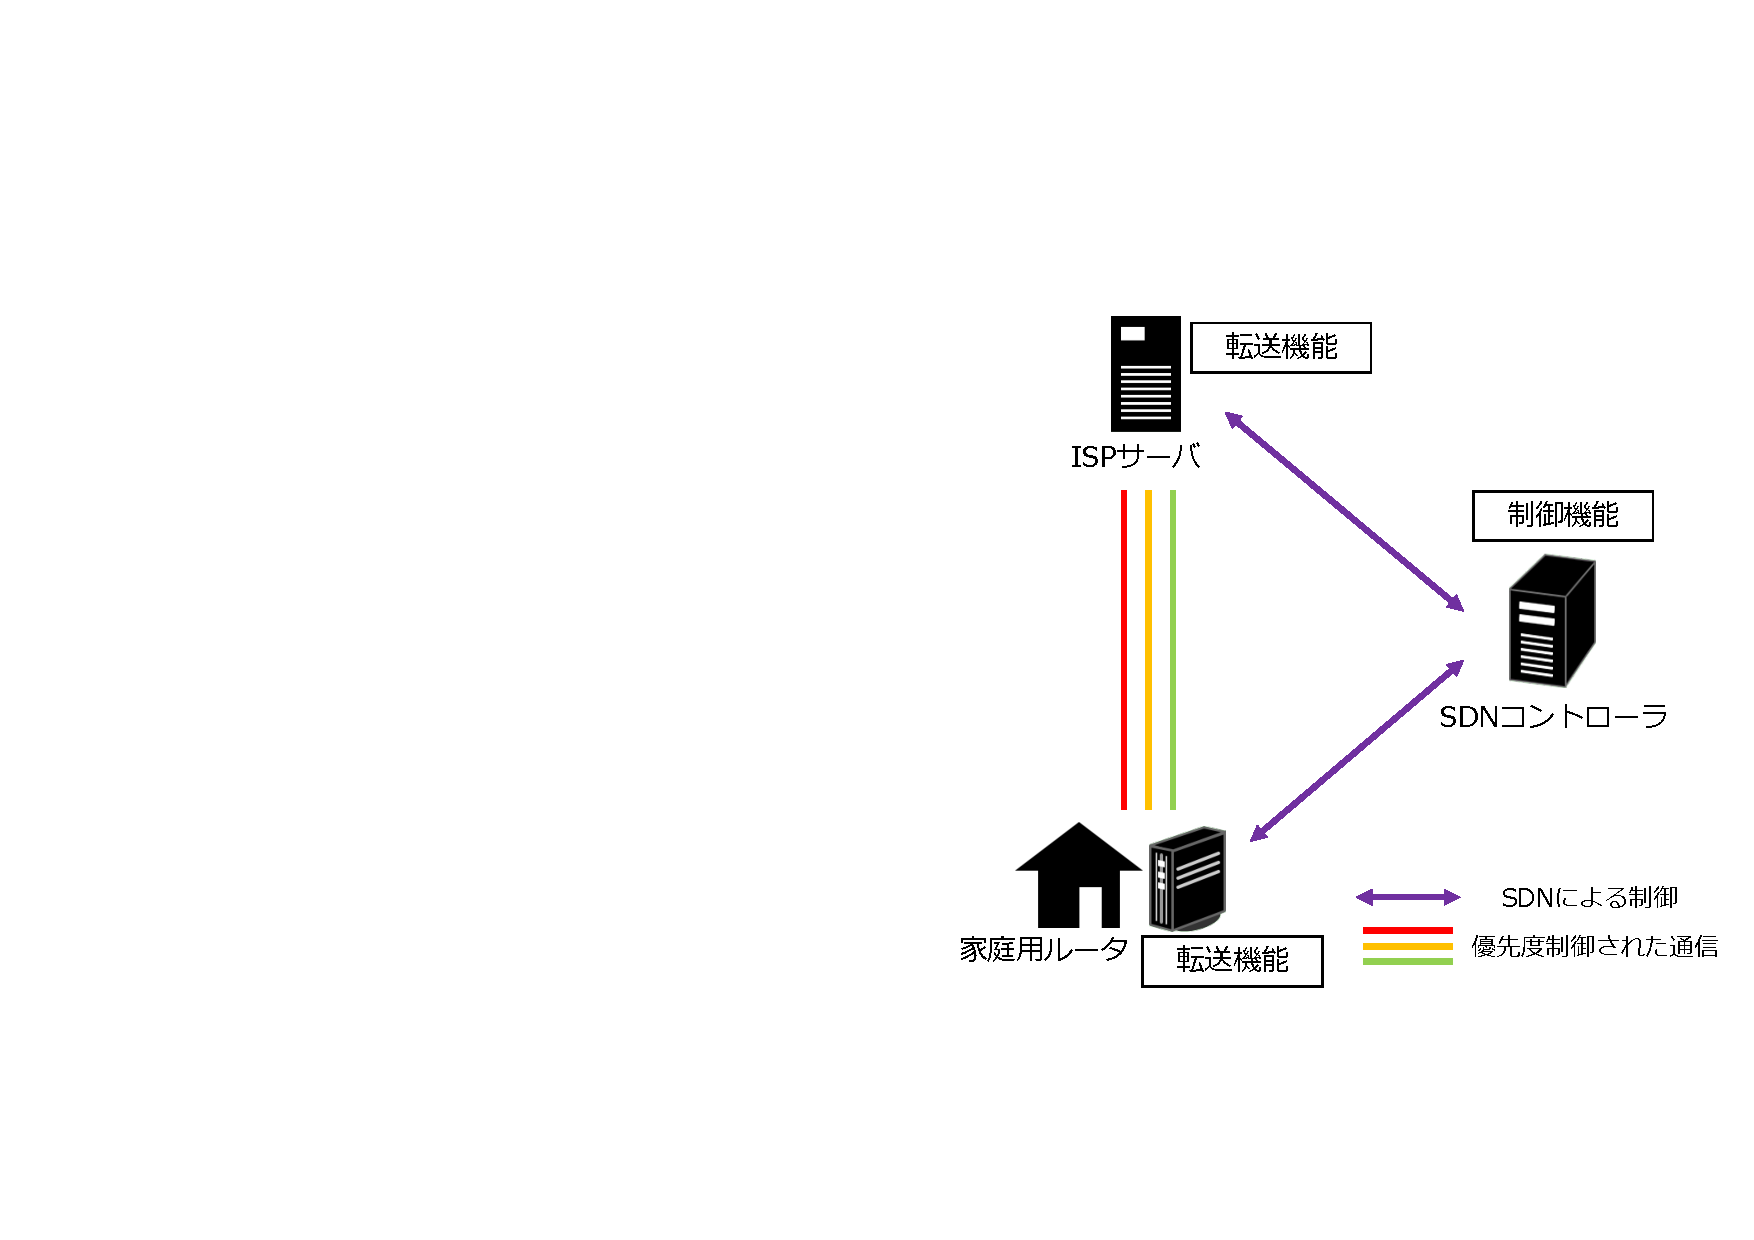
\includegraphics[width=0.7\linewidth]{img/proposal_resume.pdf}
    \caption{SDNを用いた通信制御}
    \label{fig:proposal}
    \end{centering}
\end{figure}

%---------------------------------------------------------------------
\subsection{動的な優先度設定}
\label{priority}
ホームネットワークにはデータ特性の異なる通信が混在し,ユーザや家庭の状況に応じて優先したいデータ特性は異なる.
提案手法では,優先度を決定する番号を用意し,各通信に番号を割り振ることで,通信の優先度を設定する.
番号の割り振りは状況に応じて自由に変更することができ,動的に優先度を設定することができる.
各優先度の番号には,アドミッション制御に用いる各優先度固有の重みが関連されており,番号の変更に付随して重みも変更されることで,動的な優先度制御を可能にする.

%---------------------------------------------------------------------
\subsection{アドミッション制御}
通信帯域が逼迫した場合,優先度の高い通信を送信したい時に送信できない問題が生じる.
そこで,通信帯域が逼迫した場合に,優先度の低い通信を意図的に破棄することで,優先度の高い通信のための通信帯域を確保するアドミッション制御を行う.
アドミッション制御の動作を\figref{fig:adomission}に示す.
SDNコントローラはホームネットワークとISPサーバ間の通信帯域の逼迫を検知すると,優先度の低い通信を破棄するよう家庭用ルータに指示する.
指示を受けた家庭用ルータは,優先度の低い通信を破棄する.\par
しかし,優先度のみで破棄する通信を選択すると,同じ通信が破棄され続け,通信が拒否されたことを意味する飢餓状態に陥る恐れがある.
そのため,各通信のこれまでに破棄された回数を記録しておく.
新たに通信を破棄する必要が生じた時,各通信の優先度が固有に持つ重みとこれまで破棄された回数から,新たに破棄する通信を選択する.
SDNコントローラは,選択した通信の破棄を家庭用ルータに指示し,家庭用ルータは支持された通信を破棄する.
最も優先度の低い通信も破棄の対象となることで,最も優先度の低い通信が飢餓状態に陥るのを防ぐことができる.

\begin{figure}[t]
	\begin{centering}
    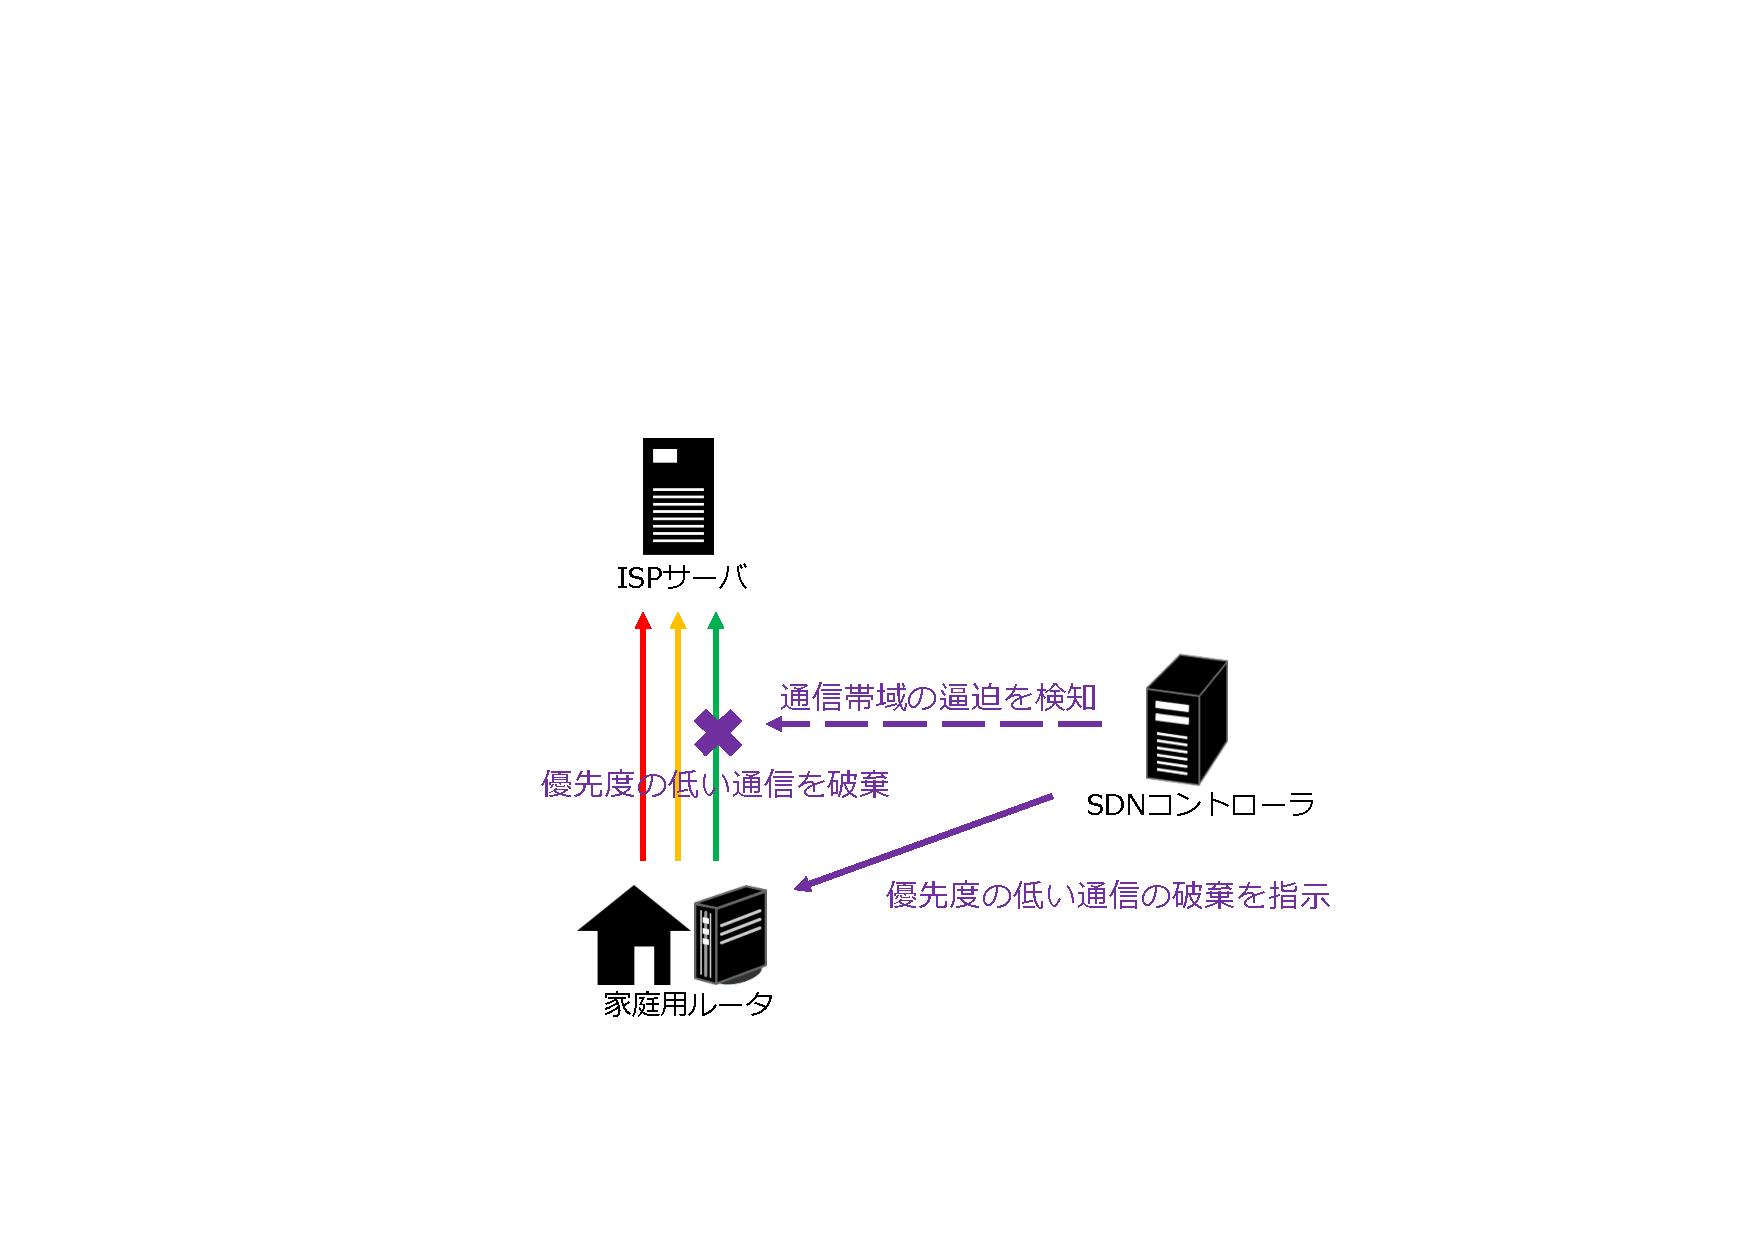
\includegraphics[width=0.8\linewidth]{img/adomission_resume.pdf}
    \caption{アドミッション制御の動作}
    \label{fig:adomission}
    \end{centering}
\end{figure}

%---------------------------------------------------------------------
\section{評価}
\subsection{実験}
提案手法を評価するにあたり,ネットワークエミュレータであるMininetを用いてホームネットワークを想定した仮想ネットワークを構築し,ネットワークシミュレーションを行う.
仮想ネットワークは,SDNコントローラ,ISPサーバ,家庭用ルータと,家庭用ルータに接続する4つのデバイスで構成される.
SDNコントローラは,SDN構築フレームワークであるRyuを用いて実装し,家庭用ルータとアドミッション制御に必要な制御メッセージをやり取りする.
家庭用ルータに接続された4つのデバイスは、カテゴリ1\textasciitilde4に分類される通信のパケットをISPサーバへ送信する.
カテゴリ1\textasciitilde4にはそれぞれ優先度1\textasciitilde4が設定されており,その優先度をもとにアドミション制御を行う.\par
提案手法の有効性を検証するため,TCP/IPパケットジェネレータおよびアナライザであるhping3を用いて,各デバイスからISPサーバまでの通信のスループットとパケットロス率を測定し,優先度が固定された既存手法と比較する.
シミュレーション途中で,優先度3=カテゴリ3と優先度4=カテゴリ4の優先度を,優先度3=カテゴリ4と優先度4=カテゴリ3に変更する.
優先度変更前と変更後でそれぞれスループットとパケットロス率を測定し,状況に応じた動的な優先度制御を行えるかを評価する.

%---------------------------------------------------------------------
\subsection{結果と考察}
優先度変更前では,既存手法,提案手法ともに優先度が高いほどスループットは高い値を示したが,優先度変更後では,\figref{fig:throughput}に示すように,既存手法では優先度3=カテゴリ4のスループットが優先度4=カテゴリ3と比較して低下しているのに対して,提案手法では優先度変更前と同様に優先度が高いほどスループットは高い値を示している.
また,優先度変更前では,既存手法,提案手法ともに優先度が低いほどパケットロス率は低い値を示したが,優先度変更後では,\figref{fig:packetloss}に示すように,既存手法では優先度3=カテゴリ4のパケットロス率が優先度4=カテゴリ3と比較して増加しているのに対して,提案手法では優先度変更前と同様に優先度が高いほどパケットロス率は低い値を示している.
以上のことから,提案手法では状況に応じた動的な優先度制御が行えていることを確認した.

\begin{figure}[t]
	\begin{centering}
    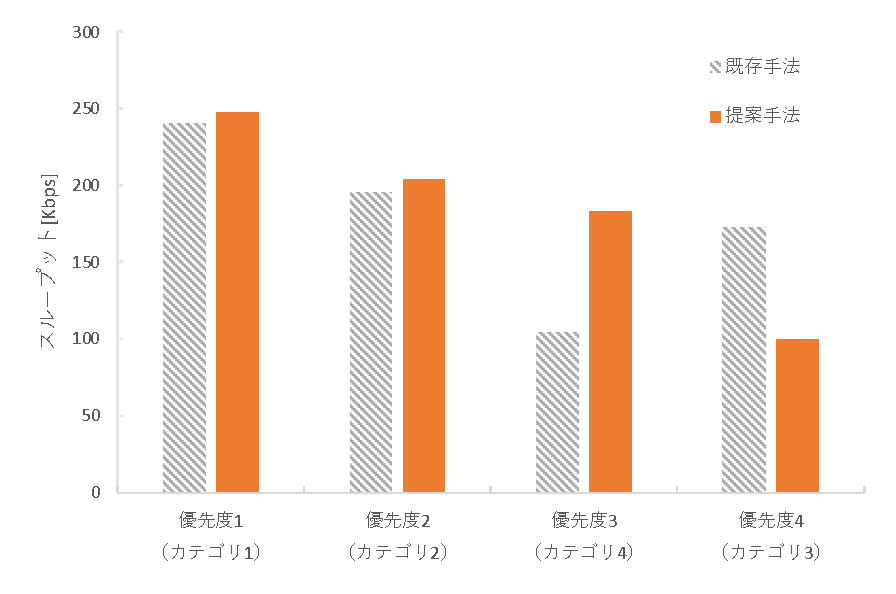
\includegraphics[width=0.88\linewidth]{img/throughput_resume.pdf}
    \caption{優先度変更後のスループット}
    \label{fig:throughput}
    \end{centering}
\end{figure}

\begin{figure}[t]
	\begin{centering}
    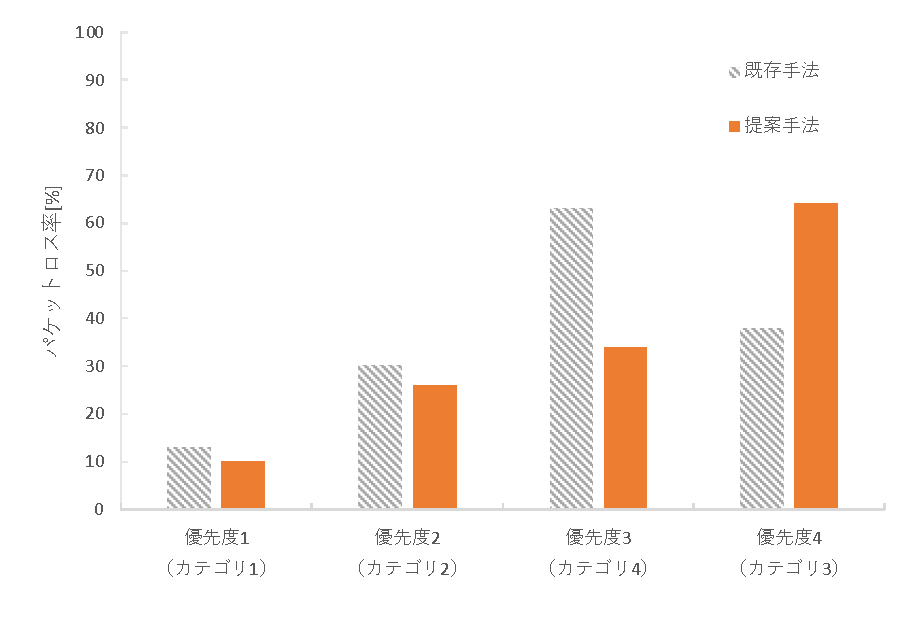
\includegraphics[width=0.88\linewidth]{img/packetloss_resume.pdf}
    \caption{優先度変更後のパケットロス率}
    \label{fig:packetloss}
    \end{centering}
\end{figure}

%---------------------------------------------------------------------
\section{まとめ}
本研究では,データ特性の異なる通信が混在するホームネットワークにおいて,通信帯域が逼迫した場合に状況に応じて優先度が高いデータを送信したい時に送信できない問題を解決するため,SDNを用いてホームネットワークとISP間の通信を制御し,通信に動的に優先度を設定し,アドミッション制御を行う手法を提案した.
提案手法について,ホームネットワークを想定した仮想ネットワークにて実験を行い,既存手法と比較して状況に応じた動的な優先度制御を行えていることを確認した.

%---------------------------------------------------------------------
% Bibliography(参考文献)
%---------------------------------------------------------------------
% thebibliography を利用する場合は以下を使用
\footnotesize{
  \begin{thebibliography}{99}
    \bibitem{ガイドライン} 総務省,帯域制御の運用基準に関するガイドライン(改定), 2019.
    \bibitem{AQRA} Guo-Cin Deng and Kuochen Wang, An Application-aware QoS Routing Algorithm for SDN-based IoT Networking, \textit{2018 IEEE Symposium on Computers and Communications (ISCC)}, pp. 186-191, 2018.
  \end{thebibliography}
}

% BibTex を利用する場合は以下を使用(初めての人には難しいかも)
% \bibliographystyle{junsrt}
% \bibliography{myref}

%---------------------------------------------------------------------
\end{document}
%---------------------------------------------------------------------
